\chapter{Related Works}
\label{chap:related works}
This study builds upon several previous works. A brief presentation of the relevant literature will aid in understanding the contributions of this thesis. This chapter provides an overview of the researches on egocentric action recognition as well as the theoretical framework of transformer-based models.

\section{Action Recognition}
\label{ar}
In many real-world applications, including gaming, \gls{hri}, and behavior analysis, it is essential to understand human actions in images or videos. Action recognition  involves identifying and localizing human behaviors. Recognizing actions in videos, particularly in real-time, is a challenging task in computer vision. Over the last decade, there has been a significant amount of research focused on action recognition using deep learning methods. Zhu et al. \cite{zhu2020comprehensive} summarized the development of deep learning methods in this area, as shown in Figure \ref{fig:summery_ar}. Karpathy et al. \cite{karpathy_large-scale_2014} introduced the DeepVideo, which was the first attempt to use \gls{cnn} to address this problem. Following this, \gls{cnn} dominated the field of action recognition for a long time. The primary advantage of this model is its ability to operate directly on raw data without any hand-crafted feature extraction.
\begin{figure}[htbp]
    \centering
    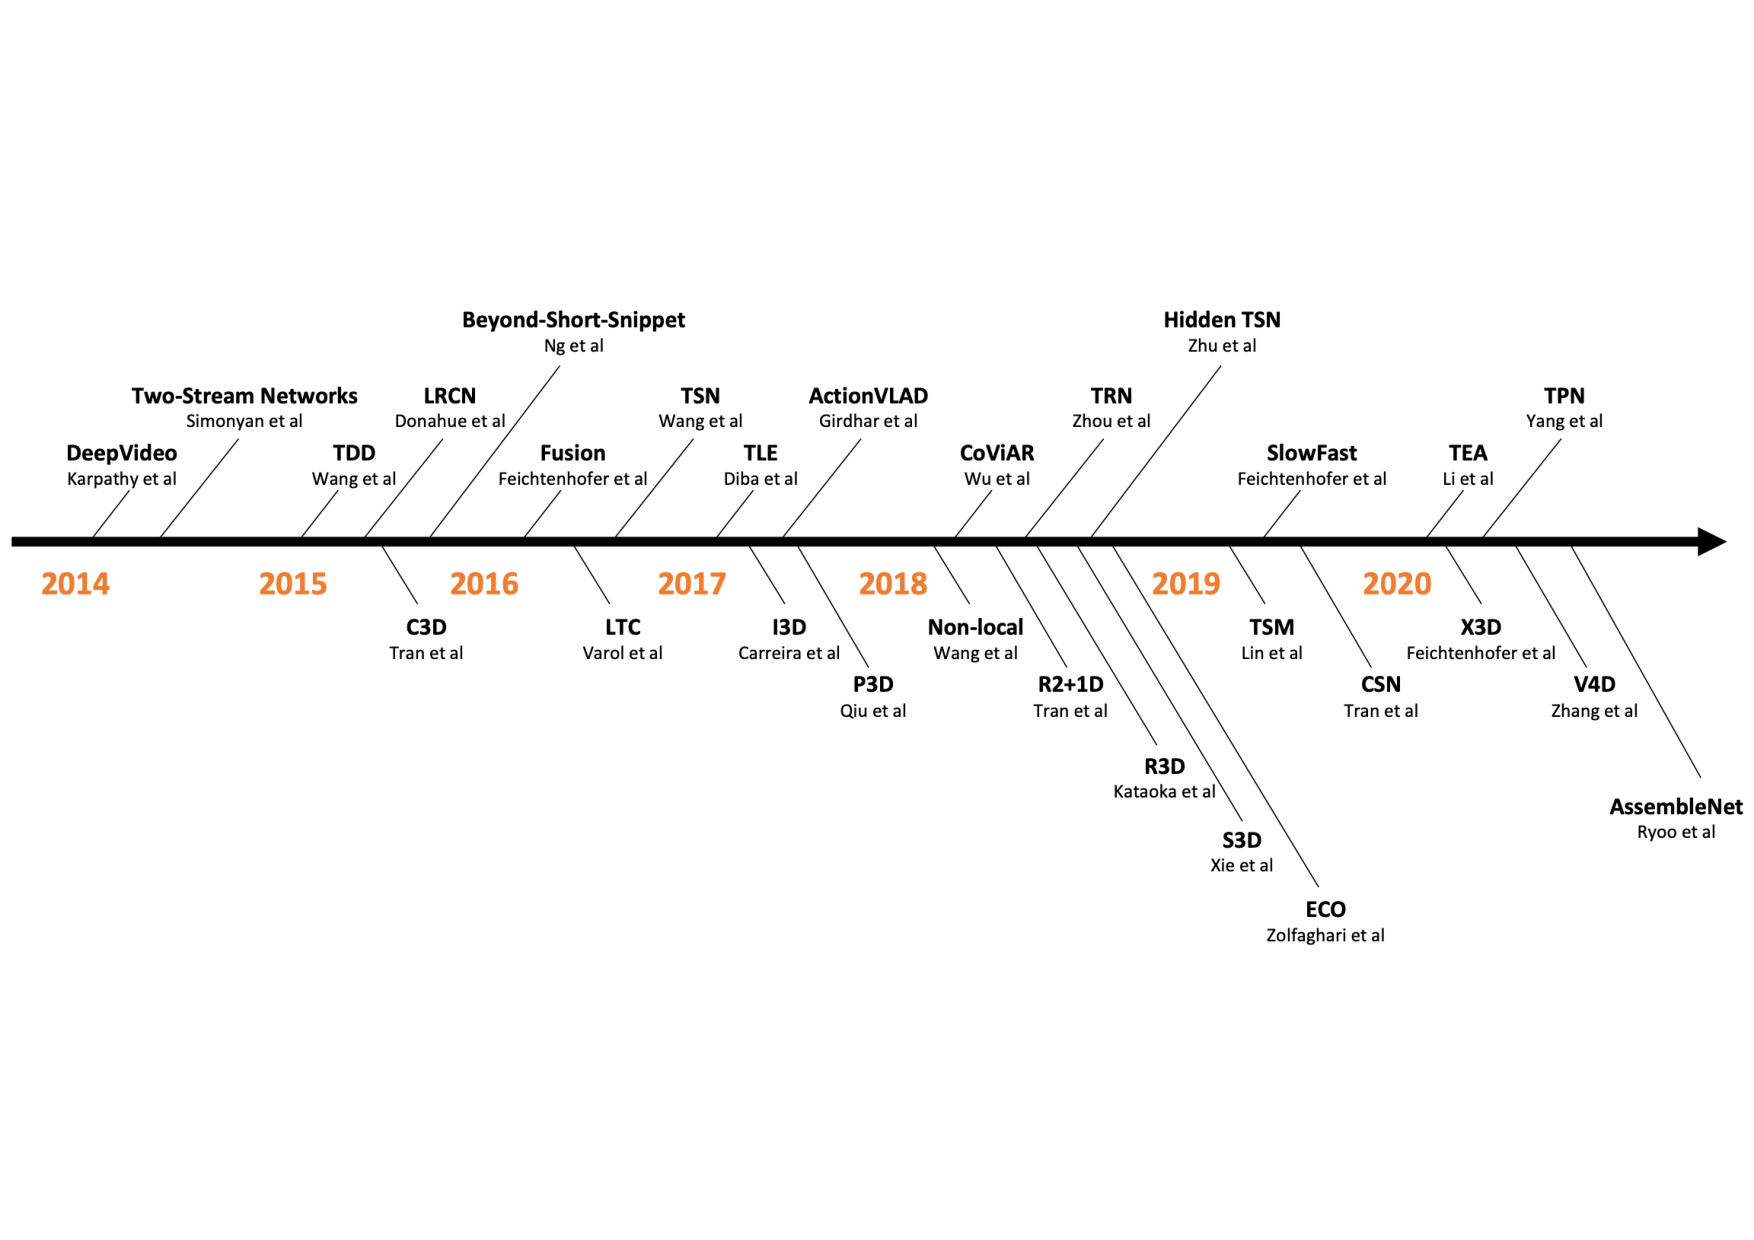
\includegraphics[width=\textwidth]{graphics/summery_ar.pdf}
    \caption{A chronological overview of representative work in video action recognition before 2020 \cite{zhu2020comprehensive}.}
    \label{fig:summery_ar}
\end{figure}

There are several challenges in developing effective video action recognition algorithms. First, some human actions are closely related and exhibit similar movement patterns, making it difficult for algorithms to distinguish between them. The second significant challenge is that the model needs to simultaneously understand both short-term information and long-term temporal information. 

Wang et al. \cite{WangXW0LTG16} proposed the \gls{tsn} to address the challenge of simultaneously understanding short-term and long-term information. The structure of \gls{tsn} is a  common example of \gls{cnn}-based models. Figure \ref{fig:tsn} shows a simplified structure of \gls{tsn}. \gls{tsn} performs video-level action recognition, by taking the entire video as input and segmenting it into several parts, uniformly distributed along the temporal dimension. \gls{tsn} then randomly selects a frame within each segment and sends it to subsequent layers. Finally, the information from the sampled frame is aggregated in the Segmental Consensus module. This segmental structure allows \gls{tsn} to observe content throughout the entire video. Many follow-up studies have handled short-term and long-term content using a similar strategy. Resently, Lin et al. \cite{lin_tsm_2019} introduced the \gls{tsm}. The part of the channels will be shifted along the temporal dimension, thereby facilitating the exchange of information among neighboring frames.

\begin{figure}
    \centering
    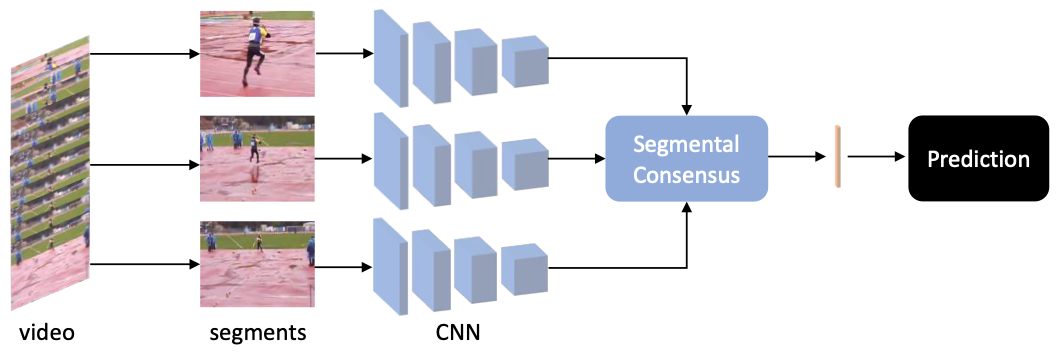
\includegraphics[width=\textwidth]{graphics/tsn.png}
    \caption{The structure of \acrfull{tsn} \cite{zhu2020comprehensive}}
    \label{fig:tsn}
\end{figure}

\section{Egocentric Action Recognition}
\label{ear}
Egocentric video, most captured by wearable cameras, are characterized by frequent and large camera movements, along with complex background scenes.
These features present unique challenges for general video transformer models.
Several high-quality egocentric video datasets have been collected in previous studies, including \cite{damen_epic-kitchens_2021}, \cite{sigurdsson_charades-ego_2018} and \cite{sigurdsson_charades-ego_2018}.
Notably, datasets such as Ego4D \cite{grauman_ego4d_2022} provide additional information like gaze, stereo and audio.
This section will review relevant research in egocentric video action recognition. 
Herzi et al. \cite{herzig_object-region_2022} proposed an object-centric module for integration with video transformers.
Wang et al. \cite{wang_symbiotic_2020} propose Symbiotic Attention with Privileged information for EAR.
Additionally, Huang et al. \cite{huang_ego-vision_2020} collected a new egocentric video dataset and developed a graphical model for joint attention detection.
Despite the progress made, previous research has often not fully addressed the specific challenges inherent in egocentric videos.
To this end, Pan et al. \cite{pan_egovit_2023} proposed a pyramid video transformer structure, showing promising results for egocentric video applications.

Other studies have focused on the role of gaze information in egocentric video.
Huang et al. \cite{huang_predicting_2018} incorporated temporal attention transition into a CNN-based saliency model for gaze estimation.
Tavakoli et al. \cite{tavakoli_digging_2019} explored both bottom-up and top-down attentional cues involved in first-person gaze guidance.
Furthermore, Lai et al. \cite{lai_eye_2022} introduces a transformer-based model that explicitly embeds global context and calculates spatio-temporal global-local correlation for egocentric gaze estimation.
In this thesis, our aim is to develop a transformer for egocentric video, building upon the EgoViT framework and incorporating DCTG with gaze information.

\section{Transformer}
\label{transformer}
Transformer is a new deep learning architecture first introduced in the paper "Attention is All You Need" by Vaswani et al. \cite{vaswani_attention_2023} in 2017. Originally used primarily for \gls{nlp} tasks, the Transformer architecture has demonstrated the ability to handle large amounts of text data effectively. Its breakthrough achievements have made Transformers a fundamental component in \gls{nlp}. The key component of the Transformer is its Attention Mechanism. The attention function is defined as mapping a query and a set of key-value pairs to an output, with the query, keys, values, and output all being vectors \cite{vaswani_attention_2023}. Figure \ref{fig:attention} visualizes the principle of the attention mechanism. The scaled dot-product attention is calculated as follows:
\begin{equation}
\text{Attention}(Q, K, V) = \text{softmax}\left(\frac{QK^T}{\sqrt{d_k}}\right) V
\end{equation}
Where $Q$ is the query, $K$ is keys, $V$ is the values, and $d_k$ is the dimension of the keys.
% \begin{figure}
%     \centering
%     \subfloat[Scaled Dot-Product Attention]{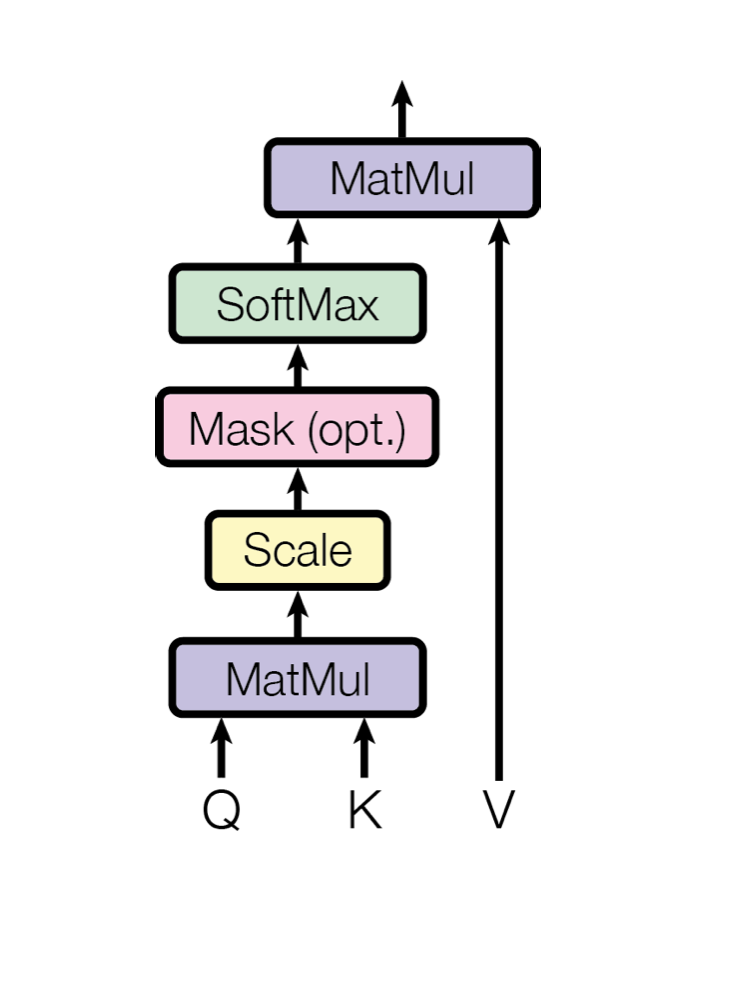
\includegraphics[width=0.4\textwidth]{graphics/attention_mech1.png}\label{fig:attention1}}
%     \hfill
%     \subfloat[Multi-Head Attention]{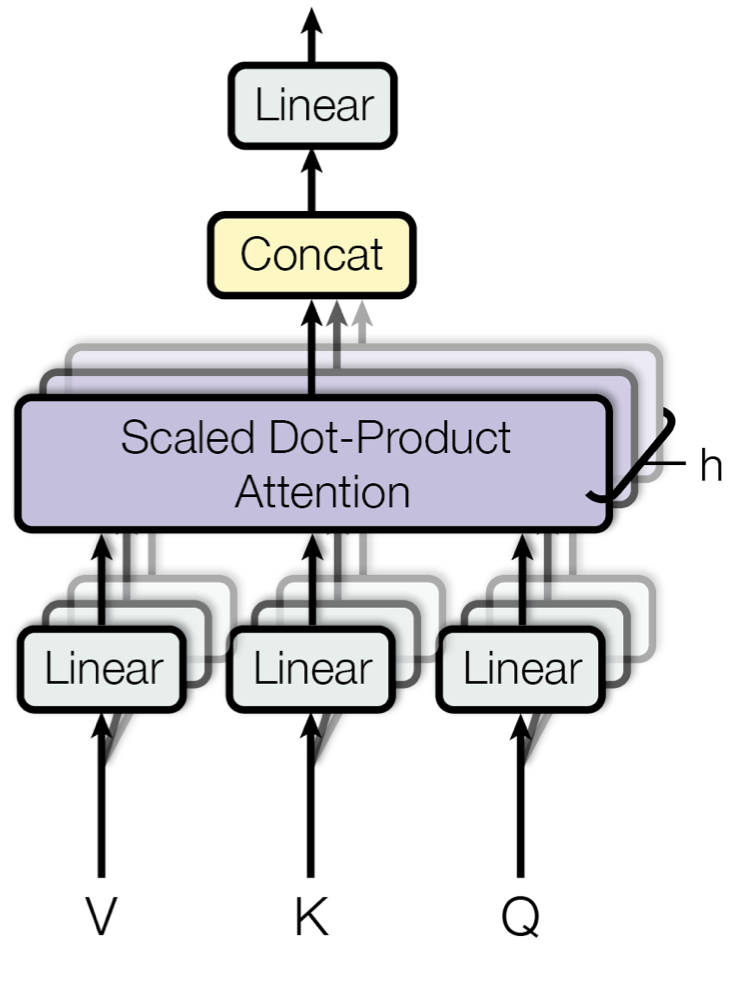
\includegraphics[width=0.4\textwidth]{graphics/attention_mech2.png}\label{fig:attention2}}
%     \caption{The schema of Scaled Dot-Product Attention Figure (a) and Multi-Head Attention Figure (b)}
%     \label{fig:attention}
% \end{figure}
\begin{figure}[htbp]
    \centering
    \subfigure[Scaled Dot-Product Attention]{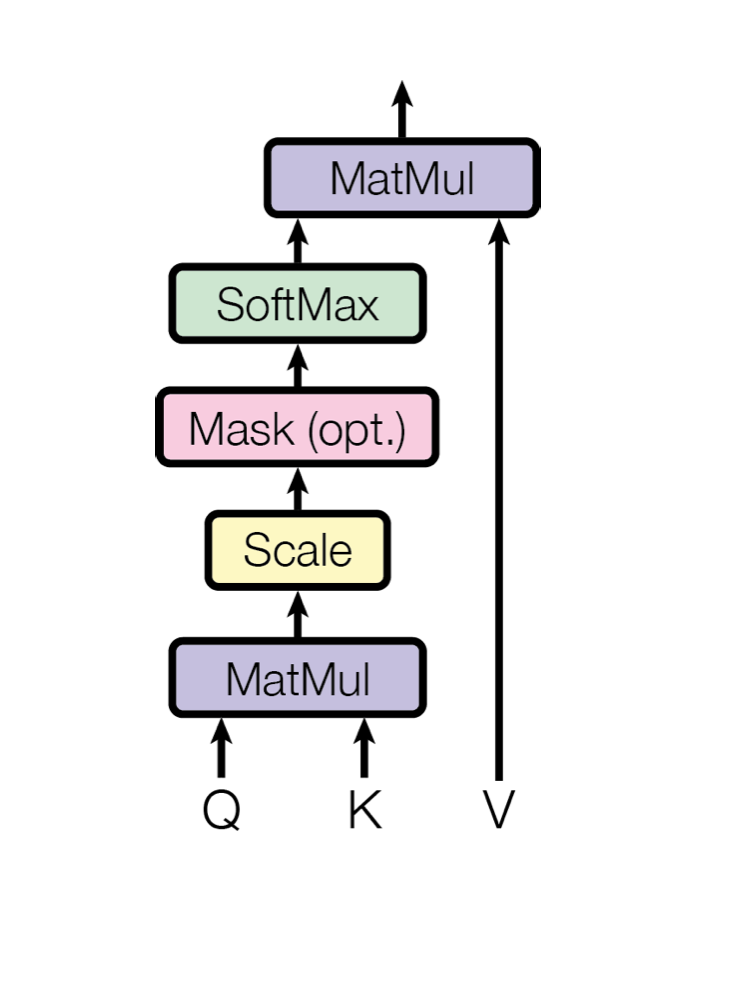
\includegraphics[width=0.4\textwidth]{graphics/attention_mech1.png}\label{fig:attention1}}
    \hfill
    \subfigure[Multi-Head Attention]{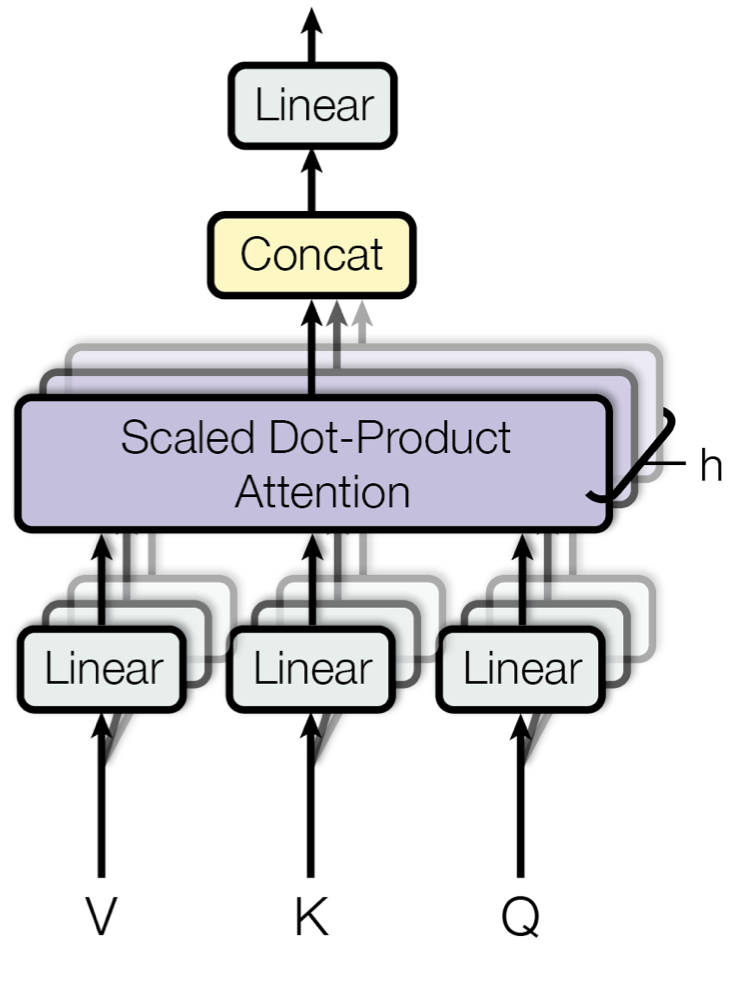
\includegraphics[width=0.4\textwidth]{graphics/attention_mech2.png}\label{fig:attention2}}
    \caption{The schema of Scaled Dot-Product Attention (a) \cite{vaswani_attention_2023} and Multi-Head Attention (b) \cite{vaswani_attention_2023}}
    \label{fig:attention}
\end{figure}
Multiple single attention function with $d_{model}$-dimension keys, values and queries are applied, and their outputs are concatenated to form the Multi-Head Attention. Hence, the Multi-Head can be described as follows:
\begin{equation}
\begin{aligned}
\text{MultiHead}(Q, K, V) &= \text{Concat}(\text{head}_1, \ldots, \text{head}_h) W^O \\
\text{where } \text{head}_i &= \text{Attention}(Q W_i^Q, K W_i^K, V W_i^V)
\end{aligned}
\end{equation}
Where $W_i^Q \in \mathbb{R}^{d_{\text{model}} \times d_k}$, $W_i^K \in \mathbb{R}^{d_{\text{model}} \times d_k}$, $W_i^V \in \mathbb{R}^{d_{\text{model}} \times d_v}$, and $W^O \in \mathbb{R}^{h d_v \times d_{\text{model}}}$.

The transformer can be divided into two parts: the Encoder and the Decoder. Each part consists of stacked identical layers, a multi-head self-attention mechanism and a feed-forward neural network. The decoder additionally includes a masked multi-head self-attention mechanism, which ensures that predictions for a given position depend only on the known outputs at previous positions \cite{vaswani_attention_2023}. The structure of the transformer is shown in Figure \ref{fig:transformer}. The self-attention mechanism has demonstrated its ability to learn the long-range dependencies. Building on the success of transformers in \gls{nlp}, several studies have explored combining \gls{cnn}-based architectures with self-attention \cite{wang_Non-local_2017}, \cite{carion_End-to-End_2020}. However, a major drawback of these models is that The global properties of self-attention may not be fully utilized during the integration of two mechanism. While they are effective at capturing local features and extracting spatial information in small areas through convolution kernels, they are less effective at capturing global information.
% Dosovitskiy et al. \cite{dosovitskiy_image_2021} proposed the \gls{vit} for image recognition. \gls{vit}, with minimal modifications from transformer, achieves excellent results compared to state-of-the-art convolutional networks. Their work has demonstrated that a pure transformer architecture is a promising solution for image recognition.
\begin{figure}
    \centering
    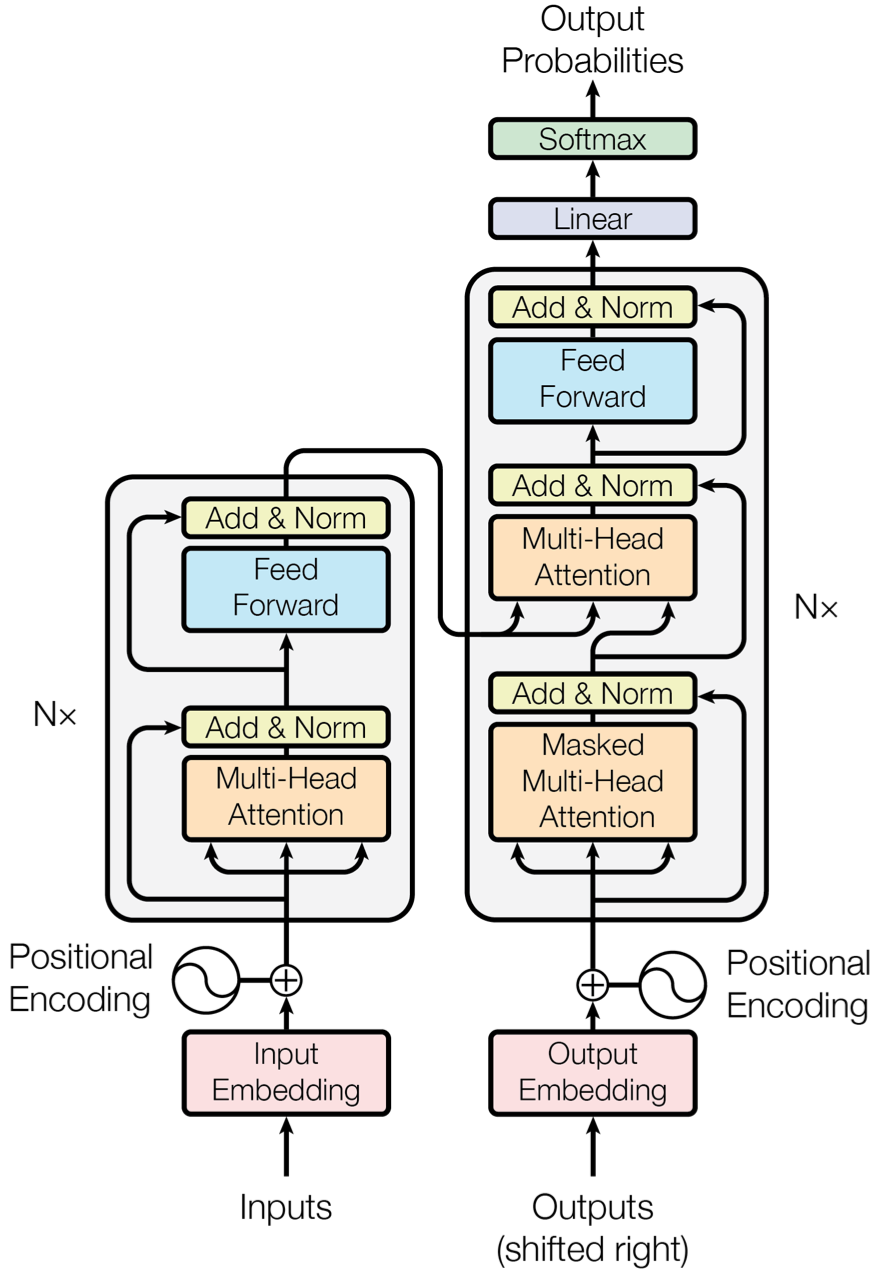
\includegraphics[width=0.6\textwidth]{graphics/structure_transformer.png}
    \caption{The structure of transformer \cite{vaswani_attention_2023}.}
    \label{fig:transformer}
\end{figure}

\section{Transformers in Video Recognition}
\label{sec:Transformers in Video Recognition}
Dosovitskiy et al. \cite{dosovitskiy_image_2021} proposed the \gls{vit} for image recognition. \gls{vit}, which globally models spatial relationships on non-overlapping image patches with minimal modifications from standard transformer \cite{vaswani_attention_2023}, achieves excellent results compared to state-of-the-art convolutional networks. Their work has demonstrated that a pure transformer architecture is a promising solution for image recognition. Following the success of \gls{vit} in image classification, multiple works have tried to explore transformer-based architectures for video recognition. Extending these advancements to video data, which adds only a spatial domain compared to image data, researchers have adapted these transformative techniques on the transformer-based model. Recently, Arnab et al. \cite{arnab_vivit_2021} presented a pure-transformer based model for video classification. The \gls{vivit} calculates a sequence of spatiotemporal tokens from input video, then processes them with self-attention. By employing several methods to factorize the model along spatial and temporal dimensions, \gls{vivit} is able to handle long-distance dependencies and complex spatiotemporal interactions effectively.

As a result, Video Transformers \cite{bertasius_is_2021}, \cite{liu_video_2021}, \cite{herzig_object-region_2022}, \cite{neimark_video_2021}, which inherit the advantages of image understanding from their predecessors, have shown remarkable success in video recognition benchmarks \cite{russakovsky_imagenet_2015}, \cite{kay_kinetics_2017}. Despite the excellent success video transformer have achieved, some video transformers like \cite{arnab_vivit_2021}, \cite{bertasius_is_2021}, \cite{neimark_video_2021} suffer from high computation costs, primarily due to extending the image spatial domain into a global spatiotemporal domain. Another disadvantage is that the performance of these video transformers heavily relies on pretrained 2D spatial models on super large dataset JFT-300M \cite{Sun_Rev_2017}. The third challenge for video transformers is the efficiency of processing long-range dependencies.  In practice, when processing long videos, important temporal information may be diluted or overshadowed by a large number of attention weights.

To address this issue, Liu et al. \cite{liu_video_2021} attempted to overcome this limitation by broadening the focus of local attention computation.
Instead of solely concentrating on the spatial domain, their approach encompasses both spatial and temporal domains. Pan et al. \cite{pan_egovit_2023} emphasize the importance of both local and global temporal attention, especially for egocentric videos, which typically contain large and frequent movements. To effectively address these problems, they proposed a pyramid structure that successfully integrates both local and global temporal attentions. This structure provides an inductive bias on grouping both local temporal attentions and the global temporal attentions \cite{pan_egovit_2023}.
In section \ref{sec:Video Swin Transformer}, the Video Swin Transformer will be discussed in detail, as it serves as the backbone of the proposed model in this thesis.

\section{Object Detection-Oriented Action Recognition}
\label{sec:Object detection-orientated video action recognition}
A number of studies \cite{ferrari_compositional_2018}, \cite{wang_symbiotic_2020}, \cite{baradel_object_2018}, \cite{xu_learning_2019} have demonstrated that models incorporating object detection and interaction features, particularly those focusing on object-human interactions, achieve considerable success in the field of video understanding.
More recently, research has focus on video action recognition with egocentric video.
Shvetsova et al. \cite{shvetsova_everything_2022} proposed a modality-agnostic transformer that integrates information from various sources into a single multi-modal representation.
Herzig et al. \cite{herzig_object-region_2022} introduced the Object-Dynamics Module, which achieved state-of-the-art performance in video action recognition.
Drawing inspiration from Herzig et al. \cite{herzig_object-region_2022}, Pan et al. \cite{pan_egovit_2023} designed the first method to incorporate object-human interaction features into a transformer.
This is achieved through a dynamic class token, embedding these features directly into the class token \cite{pan_egovit_2023}.
Their method addresses two key issues: firstly, how to incorporate object-subject interaction features, and secondly, how to embed locality inductive bias within the self-attention module.

\section{Video Swin Transformer}
\label{sec:Video Swin Transformer}
The Video Swin Transformer builds on the Swin Transformer, extending the local attention computation from solely the spatial domain to the spatiotemporal domain. The overall architecture is shown in Figure \ref{fig:swin-transformer}. Video Swin Transformer consist of four stages, each containing a patch merging layer and multiple Video Swin Transformer Block. The transformer block will be repeated $N$ times according to the model configuration. It does not down-sample along the temporal dimension, but performs $2\times$ spatial down-sampling in the patch merging layer of each stage. The input videos will be divided into several 3D patches. The patches are then processed through the stages in series. The output of the last stage is defined as the normal token, which is used for classification in subsequent head layers.
% \clearpage
\begin{figure}[htbp]
    \centering
    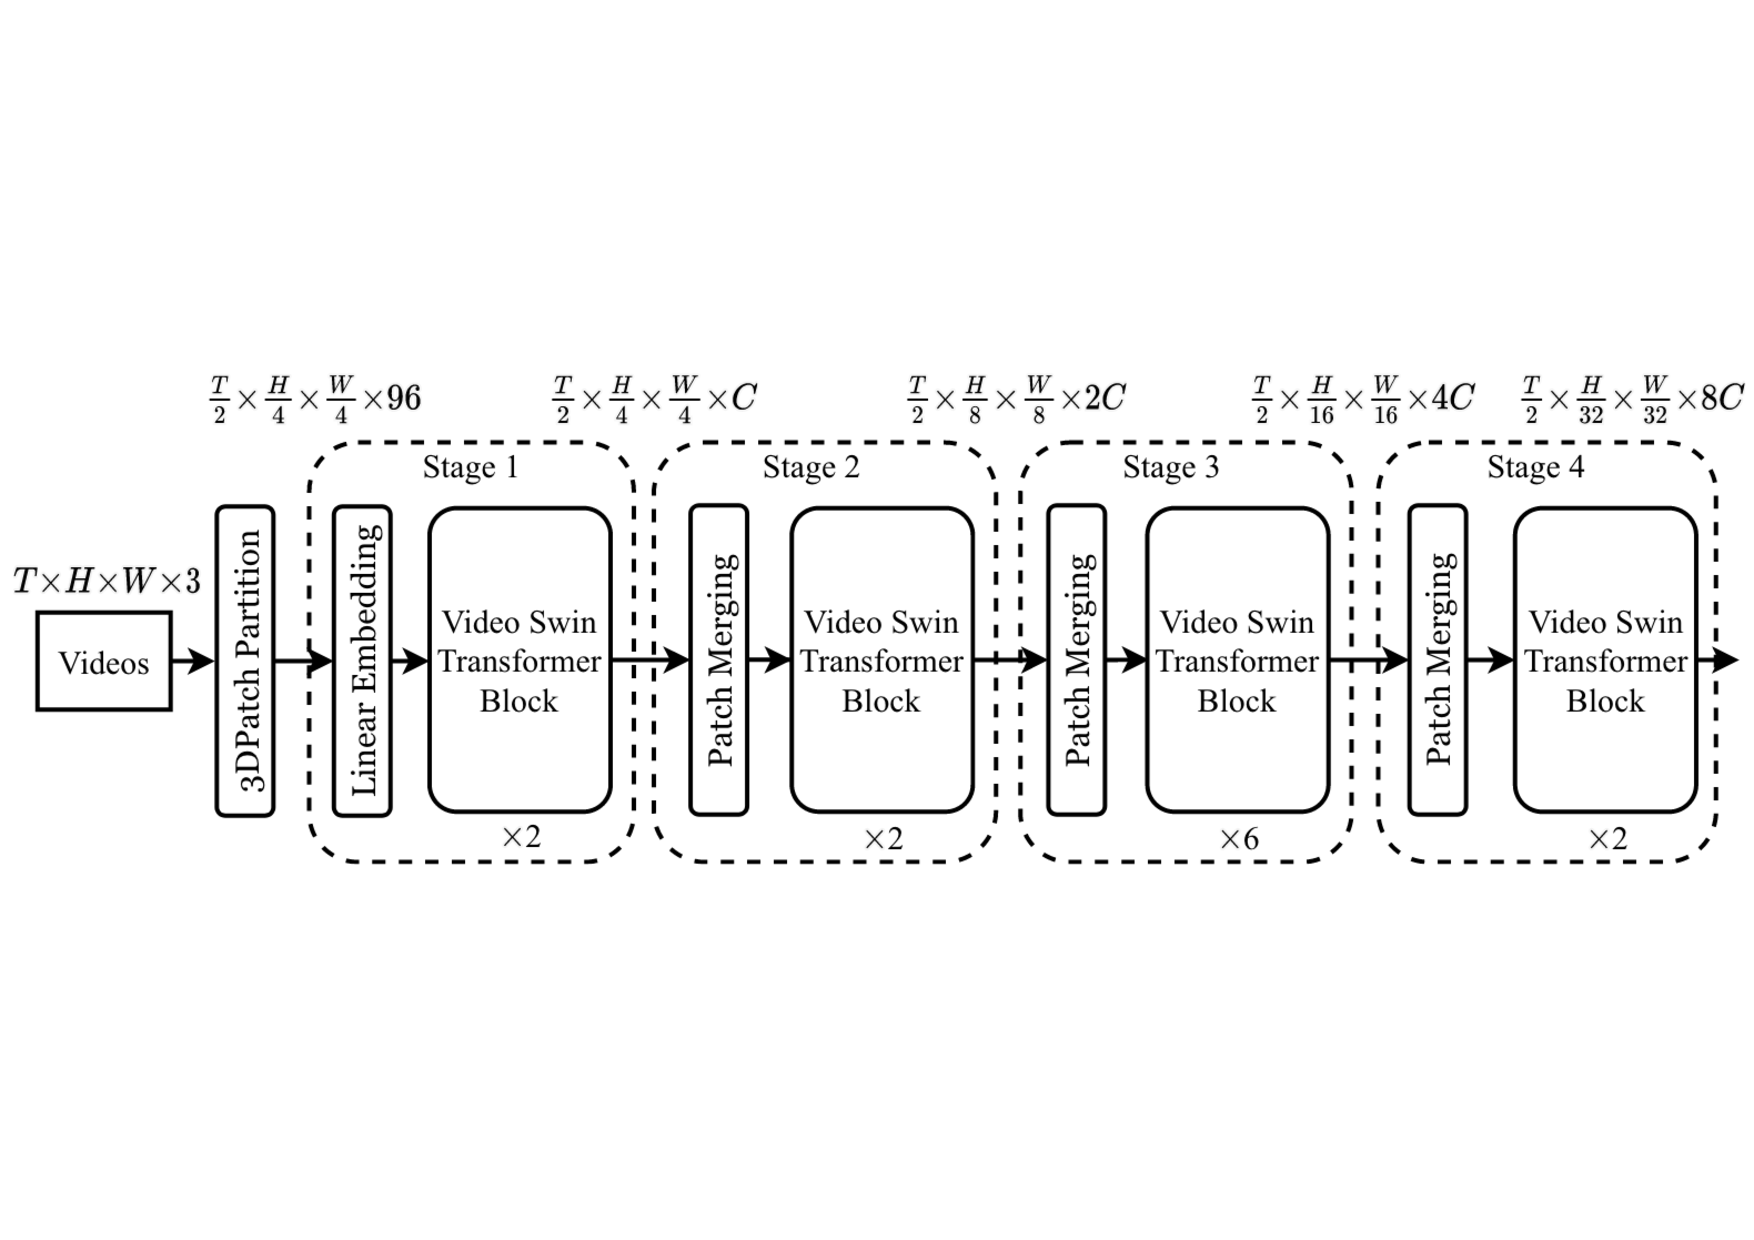
\includegraphics[width=\textwidth]{graphics/Swin_overview.pdf}
    \caption{The architecture of Video Swin Transformer (Swin-T version) \cite{liu_video_2021}.}
    \label{fig:swin-transformer}
\end{figure}

The Video Swin Transformer Block inherit the structure of standard transformer, only replacing the \gls{msa} with the 3D shifted window based multi-head self-attention module. As shown in Figure \ref{fig:swin-block}, a Video Swin Transformer Block consists of a 3D shifted windows based \gls{msa} module, a \gls{ffn}, and two \gls{ln} layers before the 3D SW-\gls{msa} and \gls{ffn}. Through the 3D shifted windows based \gls{msa}, the Video Swin Transformer introduces a locality inductive bias to the self-attention module. The shifted windows allow the non-overlapping 3D windows to exchange information with each other. Figure \ref{fig:swin-msa} illustrate the mechanism of the 3D shifted windows based \gls{msa} module. 
\vspace{5mm}

\begin{figure}[htbp]
    \centering
    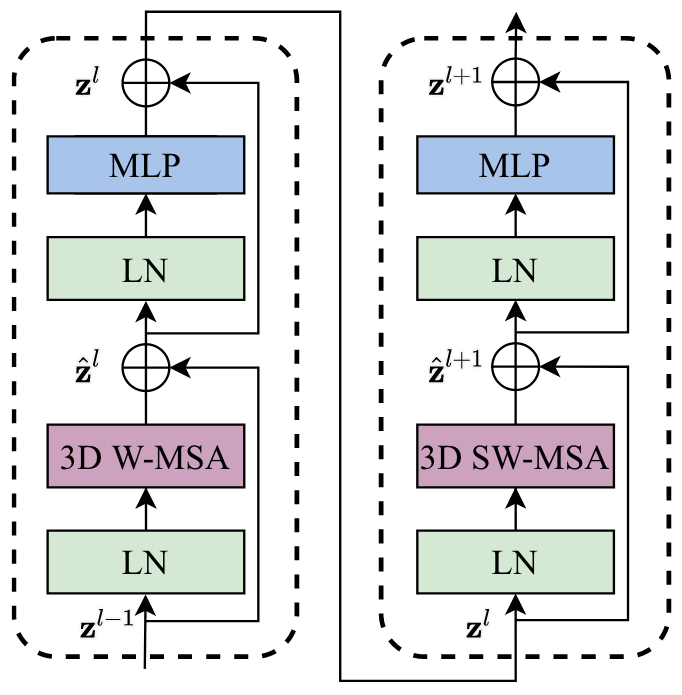
\includegraphics[width=0.5\textwidth]{graphics/swin_t_block.png}
    \caption{The structure of Video Swin Transformer Block \cite{liu_video_2021}.}
    \label{fig:swin-block}
\end{figure}
\clearpage
\vspace{5mm}
\begin{figure}[htbp]
    \centering
    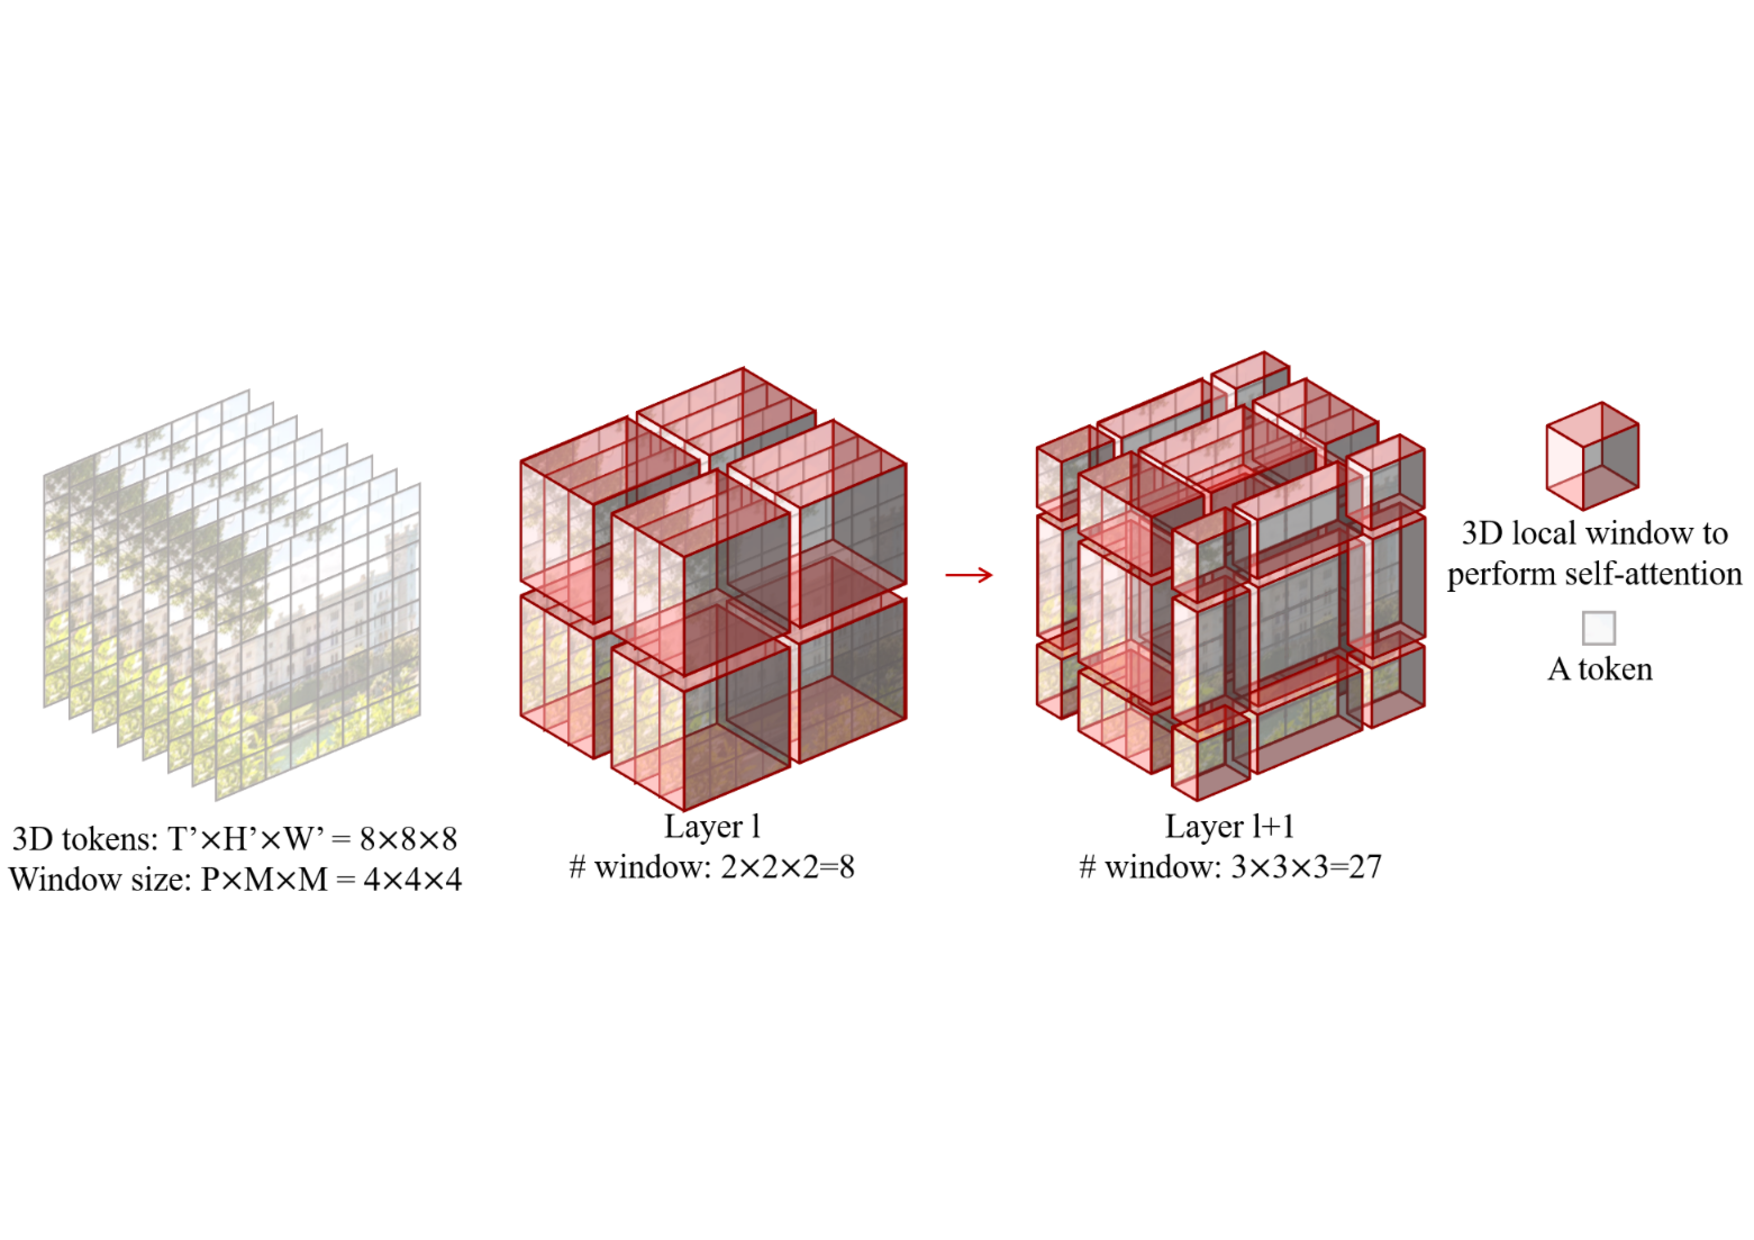
\includegraphics[width=\textwidth]{graphics/shift_window.pdf}
    \caption{The mechanism of 3D shifted windows \cite{liu_video_2021}.}
    \label{fig:swin-msa}
\end{figure}

\section{EgoViT}
\label{sec:EgoViT}
In this section, the structure and key components of EgoViT will be explained in detail. Since the proposed model in this thesis is strictly based on EgoViT, it is important to thoroughly understand the structure of EgoViT.

EgoViT features a hierarchical pyramid structure that effectively provides an inductive bias for grouping both local and global temporal attentions. This design enables it to successfully process the rapid motions typically found in egocentric videos. The overall architecture of EgoViT is shown in Figure \ref{fig:egovit}. EgoViT consists of three main parts: the Short-term Stage, Intermediate Connection and Long-term Stage.
\begin{figure}[b]
    \centering
    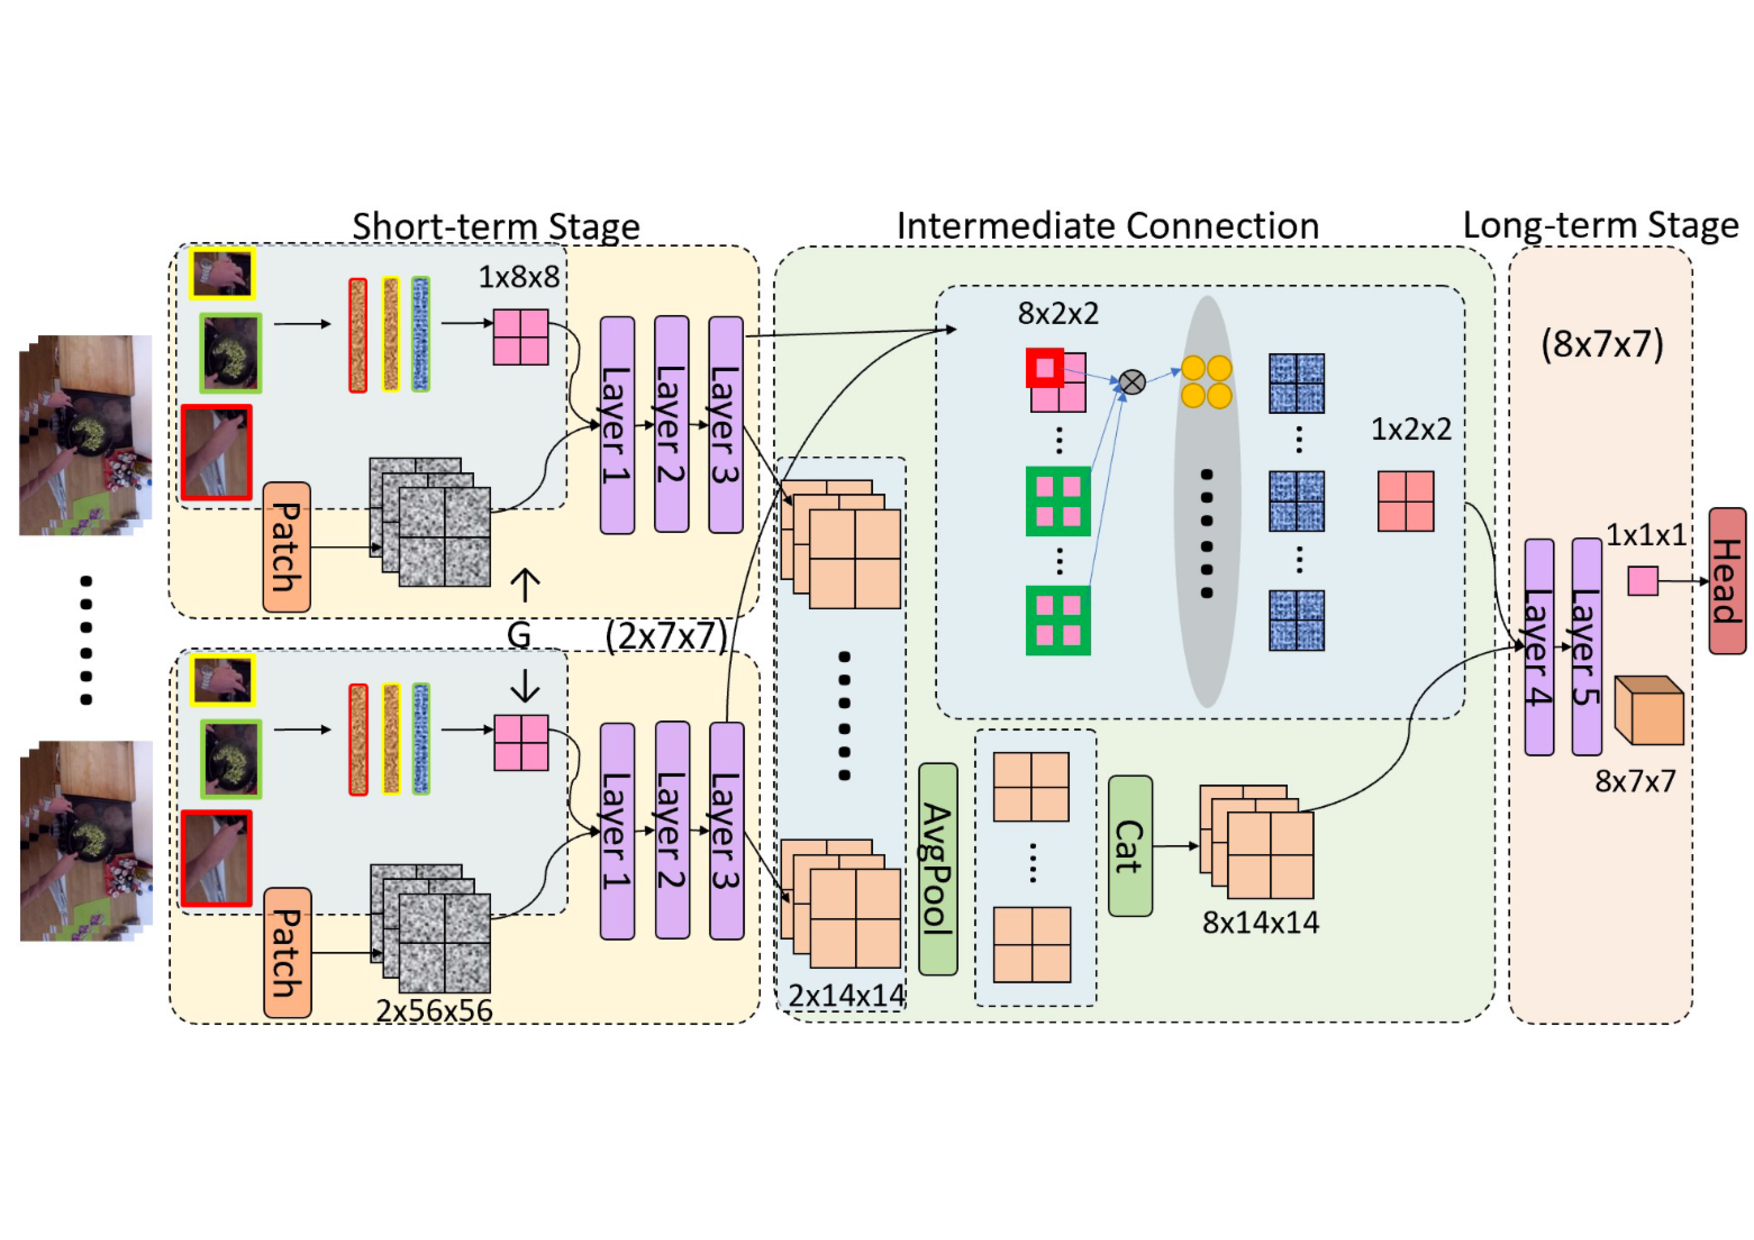
\includegraphics[width=\textwidth]{graphics/egovit.pdf}
    \caption{The architecture of EgoViT with Dynamic Class Token Generator\cite{pan_egovit_2023}.}
    \label{fig:egovit}
\end{figure}

The Short-term Stage is designed to capture the local temporal information. It is divided into $G$ groups, and each group integrates a \gls{dctg} module. The \gls{dctg} contains a pretrained \gls{hod} module, which detects the hands and objects interacting within the frames. The detected hands and objects are transformed as a combined hand-object features. These combined hand-object features are then processed in subsequent layers to generate the \gls{dct}. The \gls{dct}s are concatenated with the embedded frames for the following transformer layers. After processing in these layers, the $G$ \gls{dct}s provide a summary of the semantic meaning of each short video phase. The processed \gls{dct}s from each group are then merged in the Intermediate Connection. During this merging process, a larger weight is assigned to the \gls{dct}s that represent crucial short-term actions.
The merging process can be expressed in Eq. \ref{eq:x_cls_s}
\begin{align}
    \alpha_{g,s,g'} &= \frac{1}{\|\mathbf{x}^{cls}_{g,s}\|} \sum_{s'} \frac{\mathbf{x}^{cls}_{g,s} \cdot \mathbf{x}^{cls}_{g',s'}}{\|\mathbf{x}^{cls}_{g',s'}\|}, \notag \\
    \alpha_{g,s} &= \sum_{g' \neq g} \alpha_{g,s,g'}, \notag \\
    \mathbf{x}^{cls}_{s} &= \sum_{g} \mathbf{x}^{cls}_{g,s} \frac{\exp(\alpha_{g,s})}{\sum_{\bar{g}} \exp(\alpha_{\bar{g},s})} \label{eq:x_cls_s}
    \end{align}

Where $g$ and $g'$ are group indices, $s$ and $s'$ are spatial indices, $\alpha_{g,s,g'}$ is the score of one group, $\alpha_{g,s}$ is the total score of all groups, and $x^{cls}_s$ is the weighted class token.

The weighted class token contains information about the actions from the $G$ phases. The layers in the long-term stage aim to perceive actions over long durations and under significant scene changes by exploring the inter-relationships of the short-term actions \cite{pan_egovit_2023}. The structure of the EgoViT addresses the challenges of egocentric video action recognition, such as large-scale scene changes between distant frames and the varying contributions of nearby frames.

% \subsection{Egocentric Video Action Recognition}
% \label{Egocentric Video Action Recognition}
% Egocentric video, most captured by wearable cameras, are characterized by frequent and large camera movements, along with complex background scenes.
% These features present unique challenges for general video transformer models.
% Several high-quality egocentric video datasets have been collected in previous studies, including \cite{damen_epic-kitchens_2021}, \cite{sigurdsson_charades-ego_2018} and \cite{sigurdsson_charades-ego_2018}.
% Notably, datasets such as Ego4D \cite{grauman_ego4d_2022} provide additional information like gaze, stereo and audio.
% This section will review relevant research in egocentric video action recognition. 
% Herzi et al. \cite{herzig_object-region_2022} proposed an object-centric module for integration with video transformers.
% Wang et al. \cite{wang_symbiotic_2020} propose Symbiotic Attention with Privileged information for EAR.
% Additionally, Huang et al. \cite{huang_ego-vision_2020} collected a new egocentric video dataset and developed a graphical model for joint attention detection.
% Despite the progress made, previous research has often not fully addressed the specific challenges inherent in egocentric videos.
% To this end, Pan et al. \cite{pan_egovit_2023} proposed a pyramid video transformer structure, showing promising results for egocentric video applications.

% Other studies have focused on the role of gaze information in egocentric video.
% Huang et al. \cite{huang_predicting_2018} incorporated temporal attention transition into a CNN-based saliency model for gaze estimation.
% Tavakoli et al. \cite{tavakoli_digging_2019} explored both bottom-up and top-down attentional cues involved in first-person gaze guidance.
% Furthermore, Lai et al. \cite{lai_eye_2022} introduces a transformer-based model that explicitly embeds global context and calculates spatio-temporal global-local correlation for egocentric gaze estimation.
% In this thesis, our aim is to develop a transformer for egocentric video, building upon the EgoViT framework and incorporating DCTG with gaze information.

% \subsection{Transformers in Video Recognition}
% \label{Transformers in Video Recognition}
% Recently, Vaswani et al. \cite{vaswani_attention_2023} introduced self-attention layers, which have significantly enhanced the field of natural language processing by replacing traditional CNN and RNN layers, achieving state-of-the-art results.
% In a separate study, Dosovitskiy et al. \cite{dosovitskiy_image_2021} demonstrate that a Vision Transformer (ViT) is particularly effective for image classification tasks, especially when applied to a super large dataset such as 300M JFT \cite{Sun_Rev_2017}.
% Extending these advancements to video data, which adds only a spatial domain compared to image data, researchers have adapted these transformative techniques on the transformer-based model.
% As a result, Video Transformers \cite{arnab_vivit_2021}, \cite{bertasius_is_2021}, \cite{liu_video_2021}, \cite{herzig_object-region_2022}, \cite{neimark_video_2021}, which inherit the advantages of image understanding from their predecessors, have shown remarkable success in video recognition benchmarks \cite{russakovsky_imagenet_2015}, \cite{kay_kinetics_2017}.
% Some video transformers \cite{arnab_vivit_2021}, \cite{bertasius_is_2021}, \cite{neimark_video_2021} suffer from high computation costs, primarily due to extending the image spatial domain into a global spatio-temporal domain.
% Another disadvantage is that the performance of these video transformers heavily relies on pretrained 2D spatial models on super large dataset JFT-300M \cite{Sun_Rev_2017}.
% To address this issue, Liu et al. \cite{liu_video_2021} attempted to overcome this limitation by broadening the focus of local attention computation.
% Instead of solely concentrating on the spatial domain, their approach encompasses both spatial and temporal domains.
% Pan et al. \cite{pan_egovit_2023} emphasize the importance of both local and global temporal attention, especially for egocentric videos, which typically contain large and frequent movements.
% To effectively address these problems, they proposed a pyramid structure that successfully integrates both local and global temporal attentions.
% This structure provides an inductive bias on grouping both local temporal attentions and the global temporal attentions \cite{pan_egovit_2023}.

% \subsection{Object detection-orientated video action recognition} 
% \label{Object detection-orientated video action recognition}
% A number of studies \cite{ferrari_compositional_2018}, \cite{wang_symbiotic_2020}, \cite{baradel_object_2018}, \cite{xu_learning_2019} have demonstrated that models incorporating object detection and interaction features, particularly those focusing on object-human interactions, achieve considerable success in the field of video understanding.
% More recently, research has focus on video action recognition with egocentric video.
% Shvetsova et al. \cite{shvetsova_everything_2022} proposed a modality-agnostic transformer that integrates information from various sources into a single multi-modal representation.
% Herzig et al. \cite{herzig_object-region_2022} introduced the Object-Dynamics Module, which achieved state-of-the-art performance in video action recognition.
% Drawing inspiration from Herzig et al. \cite{herzig_object-region_2022},Pan et al. \cite{pan_egovit_2023} designed the first method to incorporate object-human interaction features into a transformer.
% This is achieved through a dynamic class token, embedding these features directly into the class token \cite{pan_egovit_2023}.
% Their method addresses two key issues: firstly, how to incorporate object-subject interaction features, and secondly, how to embed locality inductive bias within the self-attention module.

